% Standalone source for Figure: experimental workflow and model-selection protocol.
\documentclass[tikz,border=4pt]{standalone}
\usetikzlibrary{positioning,arrows.meta,fit,backgrounds}
\definecolor{blue1}{HTML}{2A78D6}
\definecolor{orange1}{HTML}{EB6834}
\definecolor{aqua1}{HTML}{1BAF7A}
\definecolor{ink2}{HTML}{52514E}
\begin{document}
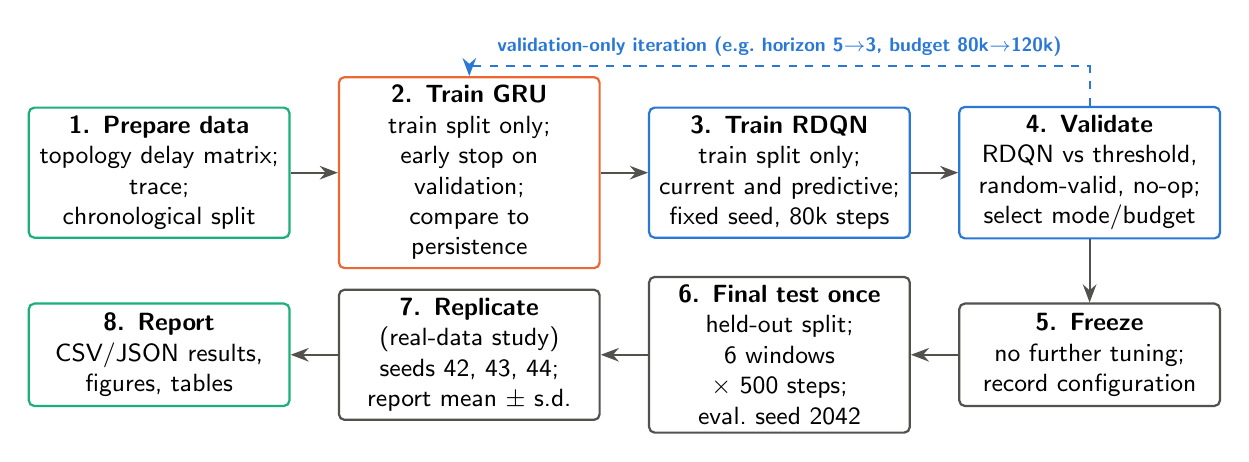
\begin{tikzpicture}[
  font=\sffamily\small,
  every node/.append style={execute at begin node={\hyphenpenalty 10000\relax}},
  step/.style={draw=#1, line width=0.8pt, rounded corners=2pt, align=center,
               fill=white, text width=31mm, minimum height=13mm, inner sep=3pt},
  step/.default=ink2,
  arr/.style={-{Stealth[length=2.3mm]}, line width=0.7pt, draw=ink2},
  tag/.style={font=\sffamily\scriptsize\bfseries, text=#1},
]
\node[step=aqua1] (a) {\textbf{1. Prepare data}\\topology delay matrix;\\trace; chronological split};
\node[step=orange1, right=6mm of a] (b) {\textbf{2. Train GRU}\\train split only;\\early stop on validation;\\compare to persistence};
\node[step=blue1, right=6mm of b] (c) {\textbf{3. Train RDQN}\\train split only;\\current and predictive;\\fixed seed, 80k steps};
\node[step=blue1, right=6mm of c] (d) {\textbf{4. Validate}\\RDQN vs threshold,\\random-valid, no-op;\\select mode/budget};
\node[step=ink2, below=8mm of d] (e) {\textbf{5. Freeze}\\no further tuning;\\record configuration};
\node[step=ink2, left=6mm of e] (f) {\textbf{6. Final test once}\\held-out split;\\6 windows $\times$ 500 steps;\\eval.\ seed 2042};
\node[step=ink2, left=6mm of f] (g) {\textbf{7. Replicate}\\(real-data study)\\seeds 42, 43, 44;\\report mean $\pm$ s.d.};
\node[step=aqua1, left=6mm of g] (h) {\textbf{8. Report}\\CSV/JSON results,\\figures, tables};
\draw[arr] (a) -- (b);
\draw[arr] (b) -- (c);
\draw[arr] (c) -- (d);
\draw[arr] (d) -- (e);
\draw[arr] (e) -- (f);
\draw[arr] (f) -- (g);
\draw[arr] (g) -- (h);
\draw[arr, dashed, draw=blue1] (d.north) -- ++(0,5mm) -| node[tag=blue1, above, pos=0.25] {validation-only iteration (e.g.\ horizon 5$\rightarrow$3, budget 80k$\rightarrow$120k)} (b.north);
\end{tikzpicture}
\end{document}
